% Options for packages loaded elsewhere
\PassOptionsToPackage{unicode}{hyperref}
\PassOptionsToPackage{hyphens}{url}
\PassOptionsToPackage{dvipsnames,svgnames,x11names}{xcolor}
%
\documentclass[
  letterpaper,
  DIV=11,
  numbers=noendperiod]{scrartcl}

\usepackage{amsmath,amssymb}
\usepackage{lmodern}
\usepackage{iftex}
\ifPDFTeX
  \usepackage[T1]{fontenc}
  \usepackage[utf8]{inputenc}
  \usepackage{textcomp} % provide euro and other symbols
\else % if luatex or xetex
  \usepackage{unicode-math}
  \defaultfontfeatures{Scale=MatchLowercase}
  \defaultfontfeatures[\rmfamily]{Ligatures=TeX,Scale=1}
\fi
% Use upquote if available, for straight quotes in verbatim environments
\IfFileExists{upquote.sty}{\usepackage{upquote}}{}
\IfFileExists{microtype.sty}{% use microtype if available
  \usepackage[]{microtype}
  \UseMicrotypeSet[protrusion]{basicmath} % disable protrusion for tt fonts
}{}
\makeatletter
\@ifundefined{KOMAClassName}{% if non-KOMA class
  \IfFileExists{parskip.sty}{%
    \usepackage{parskip}
  }{% else
    \setlength{\parindent}{0pt}
    \setlength{\parskip}{6pt plus 2pt minus 1pt}}
}{% if KOMA class
  \KOMAoptions{parskip=half}}
\makeatother
\usepackage{xcolor}
\setlength{\emergencystretch}{3em} % prevent overfull lines
\setcounter{secnumdepth}{5}
% Make \paragraph and \subparagraph free-standing
\ifx\paragraph\undefined\else
  \let\oldparagraph\paragraph
  \renewcommand{\paragraph}[1]{\oldparagraph{#1}\mbox{}}
\fi
\ifx\subparagraph\undefined\else
  \let\oldsubparagraph\subparagraph
  \renewcommand{\subparagraph}[1]{\oldsubparagraph{#1}\mbox{}}
\fi


\providecommand{\tightlist}{%
  \setlength{\itemsep}{0pt}\setlength{\parskip}{0pt}}\usepackage{longtable,booktabs,array}
\usepackage{calc} % for calculating minipage widths
% Correct order of tables after \paragraph or \subparagraph
\usepackage{etoolbox}
\makeatletter
\patchcmd\longtable{\par}{\if@noskipsec\mbox{}\fi\par}{}{}
\makeatother
% Allow footnotes in longtable head/foot
\IfFileExists{footnotehyper.sty}{\usepackage{footnotehyper}}{\usepackage{footnote}}
\makesavenoteenv{longtable}
\usepackage{graphicx}
\makeatletter
\def\maxwidth{\ifdim\Gin@nat@width>\linewidth\linewidth\else\Gin@nat@width\fi}
\def\maxheight{\ifdim\Gin@nat@height>\textheight\textheight\else\Gin@nat@height\fi}
\makeatother
% Scale images if necessary, so that they will not overflow the page
% margins by default, and it is still possible to overwrite the defaults
% using explicit options in \includegraphics[width, height, ...]{}
\setkeys{Gin}{width=\maxwidth,height=\maxheight,keepaspectratio}
% Set default figure placement to htbp
\makeatletter
\def\fps@figure{htbp}
\makeatother
\newlength{\cslhangindent}
\setlength{\cslhangindent}{1.5em}
\newlength{\csllabelwidth}
\setlength{\csllabelwidth}{3em}
\newlength{\cslentryspacingunit} % times entry-spacing
\setlength{\cslentryspacingunit}{\parskip}
\newenvironment{CSLReferences}[2] % #1 hanging-ident, #2 entry spacing
 {% don't indent paragraphs
  \setlength{\parindent}{0pt}
  % turn on hanging indent if param 1 is 1
  \ifodd #1
  \let\oldpar\par
  \def\par{\hangindent=\cslhangindent\oldpar}
  \fi
  % set entry spacing
  \setlength{\parskip}{#2\cslentryspacingunit}
 }%
 {}
\usepackage{calc}
\newcommand{\CSLBlock}[1]{#1\hfill\break}
\newcommand{\CSLLeftMargin}[1]{\parbox[t]{\csllabelwidth}{#1}}
\newcommand{\CSLRightInline}[1]{\parbox[t]{\linewidth - \csllabelwidth}{#1}\break}
\newcommand{\CSLIndent}[1]{\hspace{\cslhangindent}#1}

\usepackage{booktabs}
\usepackage{longtable}
\usepackage{array}
\usepackage{multirow}
\usepackage{wrapfig}
\usepackage{float}
\usepackage{colortbl}
\usepackage{pdflscape}
\usepackage{tabu}
\usepackage{threeparttable}
\usepackage{threeparttablex}
\usepackage[normalem]{ulem}
\usepackage{makecell}
\usepackage{xcolor}
\KOMAoption{captions}{tableheading}
\makeatletter
\makeatother
\makeatletter
\makeatother
\makeatletter
\@ifpackageloaded{caption}{}{\usepackage{caption}}
\AtBeginDocument{%
\ifdefined\contentsname
  \renewcommand*\contentsname{Table of contents}
\else
  \newcommand\contentsname{Table of contents}
\fi
\ifdefined\listfigurename
  \renewcommand*\listfigurename{List of Figures}
\else
  \newcommand\listfigurename{List of Figures}
\fi
\ifdefined\listtablename
  \renewcommand*\listtablename{List of Tables}
\else
  \newcommand\listtablename{List of Tables}
\fi
\ifdefined\figurename
  \renewcommand*\figurename{Figure}
\else
  \newcommand\figurename{Figure}
\fi
\ifdefined\tablename
  \renewcommand*\tablename{Table}
\else
  \newcommand\tablename{Table}
\fi
}
\@ifpackageloaded{float}{}{\usepackage{float}}
\floatstyle{ruled}
\@ifundefined{c@chapter}{\newfloat{codelisting}{h}{lop}}{\newfloat{codelisting}{h}{lop}[chapter]}
\floatname{codelisting}{Listing}
\newcommand*\listoflistings{\listof{codelisting}{List of Listings}}
\makeatother
\makeatletter
\@ifpackageloaded{caption}{}{\usepackage{caption}}
\@ifpackageloaded{subcaption}{}{\usepackage{subcaption}}
\makeatother
\makeatletter
\@ifpackageloaded{tcolorbox}{}{\usepackage[many]{tcolorbox}}
\makeatother
\makeatletter
\@ifundefined{shadecolor}{\definecolor{shadecolor}{rgb}{.97, .97, .97}}
\makeatother
\makeatletter
\makeatother
\ifLuaTeX
  \usepackage{selnolig}  % disable illegal ligatures
\fi
\IfFileExists{bookmark.sty}{\usepackage{bookmark}}{\usepackage{hyperref}}
\IfFileExists{xurl.sty}{\usepackage{xurl}}{} % add URL line breaks if available
\urlstyle{same} % disable monospaced font for URLs
\hypersetup{
  pdftitle={Clustering Companies by CDS Spread Curves Using Gaussian Mixture Models},
  pdfauthor={Ruizi Liu},
  colorlinks=true,
  linkcolor={blue},
  filecolor={Maroon},
  citecolor={Blue},
  urlcolor={Blue},
  pdfcreator={LaTeX via pandoc}}

\title{Clustering Companies by CDS Spread Curves Using Gaussian Mixture
Models\thanks{Code and data are available at:
\url{https://github.com/RIRI0527/437_final_project.git}.}}
\usepackage{etoolbox}
\makeatletter
\providecommand{\subtitle}[1]{% add subtitle to \maketitle
  \apptocmd{\@title}{\par {\large #1 \par}}{}{}
}
\makeatother
\subtitle{Can we identify clusters of companies that have similar risk
trends?}
\author{Ruizi Liu}
\date{April 8, 2025}

\begin{document}
\maketitle
\ifdefined\Shaded\renewenvironment{Shaded}{\begin{tcolorbox}[enhanced, frame hidden, sharp corners, borderline west={3pt}{0pt}{shadecolor}, breakable, interior hidden, boxrule=0pt]}{\end{tcolorbox}}\fi

\renewcommand*\contentsname{Table of contents}
{
\hypersetup{linkcolor=}
\setcounter{tocdepth}{3}
\tableofcontents
}
\newpage

\hypertarget{introduction}{%
\section{Introduction}\label{introduction}}

A credit default swap (CDS) is a financial swap contract. The seller of
a CDS gives the buyer indemnification in the case of a default or other
credit event by the debtor. The buyer of a CDS makes a sequence of
payments (the CDS ``premium'' or ``spread'') to the seller, and in
return, the buyer will receive a payout if the asset defaults (Wikipedia
contributors 2024). CDS are widely used as a default risk hedge for the
borrower and an arbitrage tool for investors, and are a very important
financial product in the financial markets. Barings Bank collapsed in
1995 when Nick Leeson gambled on selling straddles for derivative
securities on the Tokyo and Singapore stock exchanges and lost \$1.4
billion. Therefore, it is necessary to study which companies have the
same risk patterns according to statistical data, which can then steer
investors away from risk (Wikipedia contributors 2024). The data set
contains the CDS spreads over ten tenors (PX1 to PX10) for 600 hundreds
of firms over time (PXi is i-year tenor spread). With this richness of
structure, it is well-suited for multivariate analysis, in particular
for uncovering latent credit risk patterns.

The research question in this paper is: Can we identify clusters of
companies that have similar risk trends? More precisely, can firms be
classified into various classes according to the evaluation of the
financial market?. To solve this question, we will use Gaussian Mixture
Model (GMM), which is one of the most powerful model-based clustering
techniques.

\hypertarget{data-and-preprocessing}{%
\section{Data and Preprocessing}\label{data-and-preprocessing}}

\hypertarget{overview}{%
\subsection{Overview}\label{overview}}

The data used is from the UofT STA437 (Zwiernik 2025b), used
the\texttt{R}programming language (R Core Team 2023), the \texttt{here}
package (Müller 2023) to load the data; \texttt{dplyr} package (Wickham
et al. 2023), \texttt{mclust} package (Scrucca et al. 2023),
\texttt{knitr} package (Xie 2024) and \texttt{ggplot2} package (Wickham
2023), \texttt{psych} package (Revelle 2024), \texttt{tidyr} package
(Wickham and Henry 2024), \texttt{gridExtra} package (Auguié 2022), and
\texttt{corrplot} package (Wei and Simko 2021) to clean the data, fit
the GMM, and plot the graphs, tables and clusters.

The CDS spreads dataset contains over 1 million rows, with daily CDS
spreads (PX1 to PX10) for over 600 companies. Each row includes the
company name, ticker symbol, date, and CDS spreads for 10 maturities.
The CDS spreads (\texttt{PX1} to \texttt{PX10}) range from near-zero to
over 40,000. Table~\ref{tbl-data-summary} represents the data summary
for \texttt{PX1} to \texttt{PX10}, showed that
\texttt{PX1}--\texttt{PX10} are highly skewed with some values exceeding
40,000. Figure~\ref{fig-box-data} shows that each maturity has a wide
range and strong right skew, we use of log transformation to justify it
and handle extreme outliers. Figure~\ref{fig-cor-data} shows the
different tenors are positively correlated, but they are not perfectly
aligned, this makes multivariate modeling appropriate.

\hypertarget{tbl-data-summary}{}
\begin{longtable}[]{@{}
  >{\raggedright\arraybackslash}p{(\columnwidth - 22\tabcolsep) * \real{0.0602}}
  >{\raggedleft\arraybackslash}p{(\columnwidth - 22\tabcolsep) * \real{0.0602}}
  >{\raggedleft\arraybackslash}p{(\columnwidth - 22\tabcolsep) * \real{0.0964}}
  >{\raggedleft\arraybackslash}p{(\columnwidth - 22\tabcolsep) * \real{0.0843}}
  >{\raggedleft\arraybackslash}p{(\columnwidth - 22\tabcolsep) * \real{0.0843}}
  >{\raggedleft\arraybackslash}p{(\columnwidth - 22\tabcolsep) * \real{0.0843}}
  >{\raggedleft\arraybackslash}p{(\columnwidth - 22\tabcolsep) * \real{0.0723}}
  >{\raggedleft\arraybackslash}p{(\columnwidth - 22\tabcolsep) * \real{0.1084}}
  >{\raggedleft\arraybackslash}p{(\columnwidth - 22\tabcolsep) * \real{0.1084}}
  >{\raggedleft\arraybackslash}p{(\columnwidth - 22\tabcolsep) * \real{0.0723}}
  >{\raggedleft\arraybackslash}p{(\columnwidth - 22\tabcolsep) * \real{0.1084}}
  >{\raggedleft\arraybackslash}p{(\columnwidth - 22\tabcolsep) * \real{0.0602}}@{}}
\caption{\label{tbl-data-summary}Summary Statistics of CDS Spread
Columns (PX1--PX10)}\tabularnewline
\toprule()
\begin{minipage}[b]{\linewidth}\raggedright
\end{minipage} & \begin{minipage}[b]{\linewidth}\raggedleft
vars
\end{minipage} & \begin{minipage}[b]{\linewidth}\raggedleft
n
\end{minipage} & \begin{minipage}[b]{\linewidth}\raggedleft
mean
\end{minipage} & \begin{minipage}[b]{\linewidth}\raggedleft
sd
\end{minipage} & \begin{minipage}[b]{\linewidth}\raggedleft
median
\end{minipage} & \begin{minipage}[b]{\linewidth}\raggedleft
min
\end{minipage} & \begin{minipage}[b]{\linewidth}\raggedleft
max
\end{minipage} & \begin{minipage}[b]{\linewidth}\raggedleft
range
\end{minipage} & \begin{minipage}[b]{\linewidth}\raggedleft
skew
\end{minipage} & \begin{minipage}[b]{\linewidth}\raggedleft
kurtosis
\end{minipage} & \begin{minipage}[b]{\linewidth}\raggedleft
se
\end{minipage} \\
\midrule()
\endfirsthead
\toprule()
\begin{minipage}[b]{\linewidth}\raggedright
\end{minipage} & \begin{minipage}[b]{\linewidth}\raggedleft
vars
\end{minipage} & \begin{minipage}[b]{\linewidth}\raggedleft
n
\end{minipage} & \begin{minipage}[b]{\linewidth}\raggedleft
mean
\end{minipage} & \begin{minipage}[b]{\linewidth}\raggedleft
sd
\end{minipage} & \begin{minipage}[b]{\linewidth}\raggedleft
median
\end{minipage} & \begin{minipage}[b]{\linewidth}\raggedleft
min
\end{minipage} & \begin{minipage}[b]{\linewidth}\raggedleft
max
\end{minipage} & \begin{minipage}[b]{\linewidth}\raggedleft
range
\end{minipage} & \begin{minipage}[b]{\linewidth}\raggedleft
skew
\end{minipage} & \begin{minipage}[b]{\linewidth}\raggedleft
kurtosis
\end{minipage} & \begin{minipage}[b]{\linewidth}\raggedleft
se
\end{minipage} \\
\midrule()
\endhead
PX1 & 1 & 1061167 & 41.20 & 249.33 & 14.87 & 1.15 & 48115.24 & 48114.09
& 83.48 & 11182.56 & 0.24 \\
PX2 & 2 & 1061167 & 53.68 & 202.32 & 24.68 & 2.07 & 34522.49 & 34520.42
& 70.11 & 8620.82 & 0.20 \\
PX3 & 3 & 1061167 & 68.91 & 187.77 & 36.75 & 3.35 & 32246.85 & 32243.50
& 55.98 & 6241.14 & 0.18 \\
PX4 & 4 & 1061167 & 85.41 & 177.12 & 50.92 & 4.80 & 30048.36 & 30043.56
& 47.42 & 4992.66 & 0.17 \\
PX5 & 5 & 1061167 & 101.52 & 171.83 & 64.99 & 5.80 & 28017.64 & 28011.84
& 40.19 & 3986.23 & 0.17 \\
PX6 & 6 & 1061167 & 114.92 & 167.03 & 77.76 & 9.48 & 26671.76 & 26662.28
& 36.00 & 3457.78 & 0.16 \\
PX7 & 7 & 1061167 & 124.58 & 164.14 & 86.89 & 10.95 & 25561.03 &
25550.08 & 32.50 & 3018.35 & 0.16 \\
PX8 & 8 & 1061167 & 131.12 & 161.51 & 93.50 & 12.68 & 24590.86 &
24578.18 & 30.27 & 2736.53 & 0.16 \\
PX9 & 9 & 1061167 & 136.22 & 159.47 & 98.69 & 14.26 & 23763.96 &
23749.70 & 28.56 & 2523.28 & 0.15 \\
PX10 & 10 & 1061167 & 140.27 & 157.83 & 102.89 & 14.91 & 23052.64 &
23037.73 & 27.20 & 2356.40 & 0.15 \\
\bottomrule()
\end{longtable}

\begin{figure}

{\centering \includegraphics{437_final_project_files/figure-pdf/fig-box-data-1.pdf}

}

\caption{\label{fig-box-data}Distribution of CDS Spreads by Maturity}

\end{figure}

\begin{figure}

{\centering 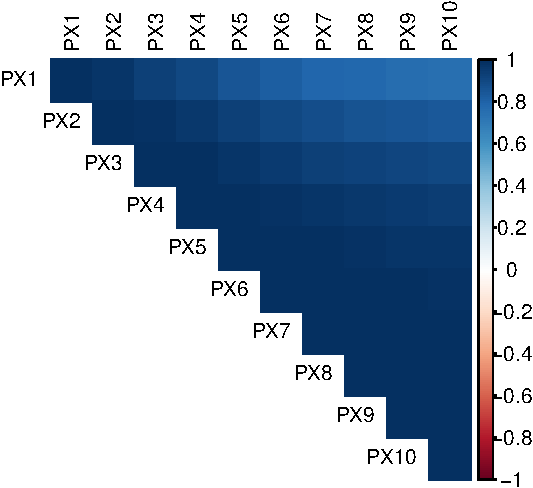
\includegraphics{437_final_project_files/figure-pdf/fig-cor-data-1.pdf}

}

\caption{\label{fig-cor-data}Correlation Between CDS Spread Tenors}

\end{figure}

\hypertarget{data-cleaning-transformation}{%
\subsection{Data Cleaning \&
Transformation}\label{data-cleaning-transformation}}

We first use \texttt{anyNA()} to check if there is NAs in the data, we
got the return \texttt{FALSE} so there is no NAs. Next, we compute the
average CDS spreads over time per company to create a single CDS spreads
curve per firm, and apply the \texttt{log1p()} fuction to transform the
data, this is to reduce skew. Then standardized each \texttt{PXi} column
using \texttt{scale()} function to ensure comparability across
dimensions.

\hypertarget{methodology}{%
\section{Methodology}\label{methodology}}

We select GMM for application in cluster analysis. In comparison with
other cluster analysis methods, for example, k-mean clustering or
hierarchical clustering, clusters in GMM can assume more flexible
directions, shapes, and covariance structures. GMM is thus better
adapted to capture the term structure of credit default swaps (CDS).
Moreover, GMM offers soft probability assignments and automatic model
selection through Bayesian Information Criterion (BIC), and it is thus a
more robust and explanatory option.

We applied Gaussian Mixture Models (GMMs) to the transformed, averaged
CDS spread data, which follows the standardized noral distribution. We
assume each company's CDS spread curve (a 10-dimensional vector of
PX1--PX10) comes from one of K unknown groups, each modeled by a
multivariate normal distribution. This followed by the mixture model: \[
p(x_i) = \sum_{k=1}^{K} \pi_k \cdot \mathcal{N}(x_i \mid \mu_k, \Sigma_k)
\] where

\begin{itemize}
\item
  \(\pi_k\) is the mixing proportion for cluster \(k\), with
  \(\sum_k \pi_k = 1\),
\item
  \(\mathcal{N}(x_i \mid \mu_k, \Sigma_k)\) is the multivariate Gaussian
  pdf for cluster \(k\),
\item
  \(\mu_k\) and \(\Sigma_k\) are the mean and covariance matrix of
  cluster \(k\).
\end{itemize}

Since our goal is to find cluster for each company, so we do not know
the cluster for each company, thus, it is latent. We can apply the EM
Algorithm (Expectation-Maximization) to estimate the parameters and
assign clusters. We use \texttt{Mclust()} function to choose the \(K\)
automatically by BIC, in Section~\ref{sec-add-fig-tbl},
Figure~\ref{fig-BIC} will show a bar plot where the best \(K\) is the
one with the highest BIC score. For each \(K\), it fits a GMM and
compute it BIC, the \texttt{Mclust()} function will select the model
with the highest BIC value, which has the best balance of fit and
simplicity. Then we randomly initialize the means \(\mu_k\), covariance
\(\Sigma_k\), and mixing proportion \(\pi_k\). This is also automaticlly
done by the \texttt{Mclust()} function.

Next we move to the E-Step (Expectation). We need to compute the
posterior probability that observation \(x_i\) belongs to cluster \(k\):
\[
\gamma_k^{(t)}(x_i) = P(Z_i = k \mid x_i) = 
\frac{ \pi_k^{(t)} \cdot \mathcal{N}(x_i \mid \mu_k^{(t)}, \Sigma_k^{(t)}) }
     { \sum_{j=1}^{K} \pi_j^{(t)} \cdot \mathcal{N}(x_i \mid \mu_j^{(t)}, \Sigma_j^{(t)}) }
\] This gives a posterior probability (or responsibilities) that each
point \(x_i\) belongs to cluster \(k\). These responsibilities are then
used to form the expected complete-data log-likelihood: \[
Q(\theta; \theta^{(t)}) = \sum_{i=1}^{n} \sum_{k=1}^{K} \gamma_k(x_i) \left[ \log \mathcal{N}(x_i \mid \mu_k, \Sigma_k) + \log \pi_k \right]
\]

In the M-Step (Maximazation), we will updating the parameters in our
model by maximizing the log-likelihood \(Q(\theta; \theta^{(t)})\),
which is obtained in the E-Step already. The parameters need to be
updated are mixing proportions \(\pi_k\), the cluster mean \(\mu_k\),
and the covariance matrix \(\Sigma_k\). We using the current
responsibilities \(\gamma_k(x_i)\) as werights:

\begin{itemize}
\tightlist
\item
  Updating mixing proportions \(\pi_k\): \[
  \pi_k^{(t+1)} = \frac{1}{n} \sum_{i=1}^{n} \gamma_k^{(t)}(x_i)
  \]
\item
  Updating cluster mean \(\mu_k\): \[
  \mu_k^{(t+1)} = \frac{\sum_{i=1}^{n} \gamma_k^{(t)}(x_i) \cdot x_i}{\sum_{i=1}^{n} \gamma_k^{(t)}(x_i)}
  \]
\item
  Updating covariance matrix \(\Sigma_k\): \[
  \Sigma_k^{(t+1)} = \frac{\sum_{i=1}^{n} \gamma_k^{(t)}(x_i) (x_i - \mu_k^{(t+1)})(x_i - \mu_k^{(t+1)})^\top}{\sum_{i=1}^{n} \gamma_k^{(t)}(x_i)}
  \]
\end{itemize}

These updated parameters will be used in the next E-Step, the EM
algorithm iterates between the E-step and M-step until convergence, at
which point the log-likelihood no longer increases significantly (i.e.,
the log-likelihood stabilize) (Zwiernik 2025a).

Once the converged in the EM Algorithm, we can assign each \(x_i\) in
data to the cluster with highest posterior probability \[
\hat{z}_i = \arg\max_k \, \gamma_k(x_i),
\] which give us the final clusters.

\hypertarget{sec-result}{%
\section{Results}\label{sec-result}}

\hypertarget{model-visualization}{%
\subsection{Model Visualization}\label{model-visualization}}

Section~\ref{sec-result} represents the key findings. We apply the
\texttt{Mclust()} function to fit our GMM automatically,
Table~\ref{tbl-model-sum} reports the estimated means (PX1--PX10) and
blending percentages for the clusters detected by the GMM. Cluster 3,
which contains 17.4\% of companies, has the highest mean CDS spreads
over tenors, pointing to high credit risk. Cluster 1 and Cluster 5 have
negative average values, which correspond to better credit profiles.
Cluster 4, the most frequent group (27.5\%), has close-to-zero spread
values, which suggest base creditworthiness. These cluster profiles
confirm that GMM successfully captured important variation in firm risk
profiles from multivariate CDS term structure data.

Table~\ref{tbl-cluster-summary} represents the number of companies
allocated to each risk cluster by the Gaussian Mixture Model. Cluster 4
has the highest number of companies (197), and Cluster 2 is the smallest
cluster (18 companies), which would suggest that it could be a rare or
transitional risk profile.

\hypertarget{tbl-model-sum}{}
\begin{longtable}[]{@{}lrrrrrrrrrrr@{}}
\caption{\label{tbl-model-sum}GMM Coefficient Summary
Table}\tabularnewline
\toprule()
Cluster & Proportion & PX1 & PX2 & PX3 & PX4 & PX5 & PX6 & PX7 & PX8 &
PX9 & PX10 \\
\midrule()
\endfirsthead
\toprule()
Cluster & Proportion & PX1 & PX2 & PX3 & PX4 & PX5 & PX6 & PX7 & PX8 &
PX9 & PX10 \\
\midrule()
\endhead
1 & 0.256 & -0.518 & -0.549 & -0.568 & -0.571 & -0.574 & -0.583 & -0.589
& -0.590 & -0.590 & -0.591 \\
2 & 0.028 & -0.285 & -0.355 & -0.410 & -0.466 & -0.532 & -0.575 & -0.579
& -0.582 & -0.575 & -0.573 \\
3 & 0.174 & 0.793 & 0.835 & 0.883 & 0.921 & 0.950 & 0.971 & 0.981 &
0.987 & 0.989 & 0.991 \\
4 & 0.275 & 0.023 & 0.036 & 0.011 & 0.002 & -0.015 & -0.022 & -0.028 &
-0.030 & -0.032 & -0.034 \\
5 & 0.103 & -0.755 & -0.720 & -0.605 & -0.554 & -0.462 & -0.379 & -0.336
& -0.318 & -0.306 & -0.297 \\
6 & 0.164 & 0.453 & 0.425 & 0.383 & 0.339 & 0.294 & 0.255 & 0.234 &
0.222 & 0.216 & 0.212 \\
\bottomrule()
\end{longtable}

\hypertarget{tbl-cluster-summary}{}
\begin{longtable}[]{@{}lr@{}}
\caption{\label{tbl-cluster-summary}Number of Companies per GMM
Cluster}\tabularnewline
\toprule()
Cluster & Number\_of\_Companies \\
\midrule()
\endfirsthead
\toprule()
Cluster & Number\_of\_Companies \\
\midrule()
\endhead
1 & 163 \\
2 & 18 \\
3 & 110 \\
4 & 197 \\
5 & 69 \\
6 & 104 \\
\bottomrule()
\end{longtable}

In Figure~\ref{fig-cluster}, we plotted the clustering outcomes on PX1
(short-run spread) and PX10 (long-run spread) as axes. To aid
interpretability, we superimposed ellipses for the variance and
correlation structure of the modeled Gaussian components of the GMM. The
figure emphasizes both the different risk profiles of the clusters and
also the soft probabilistic boundaries between the clusters. For
example, clusters with high PX1 and PX10 (e.g., Cluster 3) are those of
companies with consistently high credit risk, while others (e.g.,
Cluster 1) group companies with relatively low spreads and flat term
structures. In Section~\ref{sec-add-fig-tbl},
Table~\ref{tbl-top-5-companies} represents the list of top 5 companies
from each cluster.

\begin{figure}

{\centering 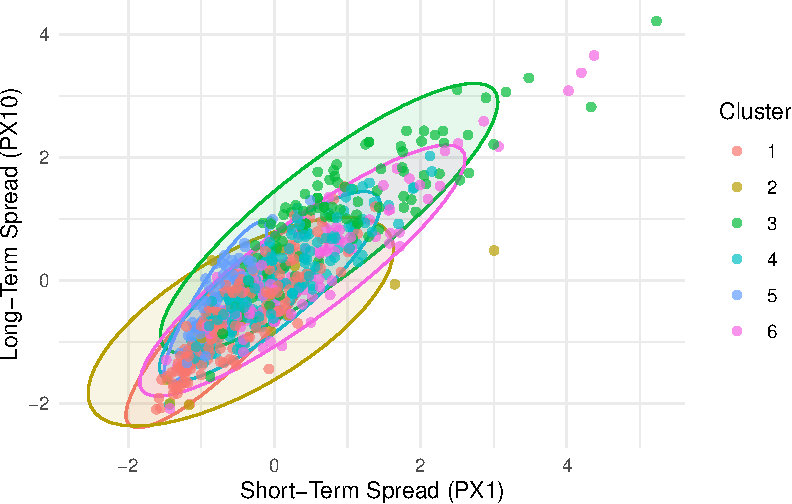
\includegraphics{437_final_project_files/figure-pdf/fig-cluster-1.pdf}

}

\caption{\label{fig-cluster}Clusters of CDS Spread Curves}

\end{figure}

\hypertarget{result-analysis}{%
\subsection{Result Analysis}\label{result-analysis}}

\begin{figure}

{\centering 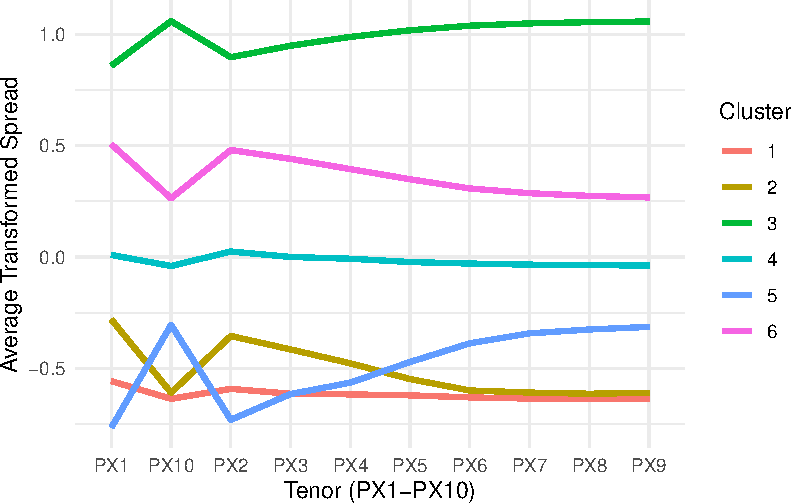
\includegraphics{437_final_project_files/figure-pdf/fig-trend-1.pdf}

}

\caption{\label{fig-trend}CDS Term Structure by Cluster}

\end{figure}

In Figure~\ref{fig-trend}, the term structure of credit default swap
(CDS) spreads (from PX1 to PX10) varies considerably across clusters.
Cluster 3 consistently experiences the highest spreads across all
maturities, suggesting that these companies carry persistently higher
credit risks. Cluster 1 and Cluster 2 exhibit lower spreads and
relatively flat curves, indicating a more stable credit profile. These
characteristics represent compelling evidence that GMM identifies
economically relevant risk groupings.

\begin{figure}

{\centering 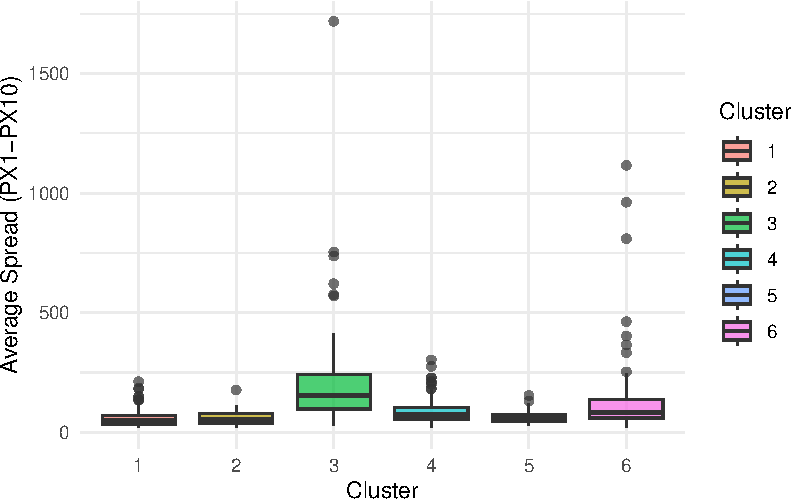
\includegraphics{437_final_project_files/figure-pdf/fig-boxplot-1.pdf}

}

\caption{\label{fig-boxplot}Boxplot of Average CDS Spread by Cluster}

\end{figure}

In Figure~\ref{fig-boxplot}, the box plots of the CDS spread averages
show that the clusters differ by the level of credit risk. Cluster 3
contains the most risky firms, followed by cluster 6, which is riskier.
Clusters 1, 2 and 5 present a lower and narrower spread distribution,
i.e., they consist of less risky firms. These findings are in line with
the spread curve analysis and confirm the reasonableness of the cluster
analysis.

\begin{figure}

{\centering 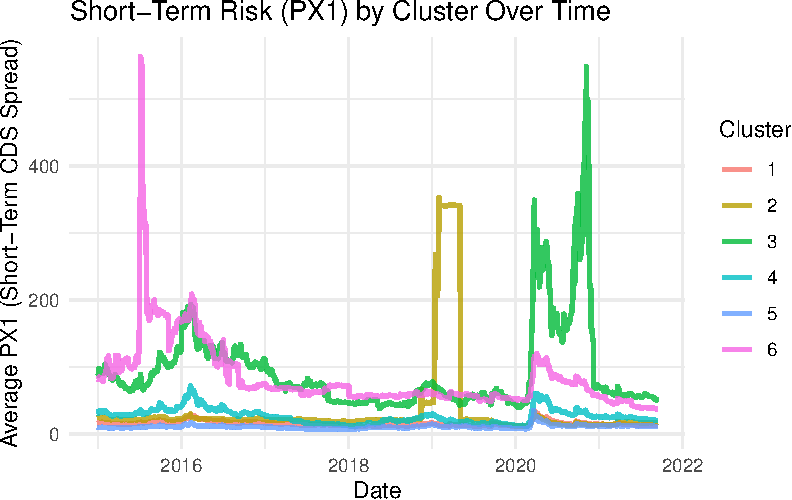
\includegraphics{437_final_project_files/figure-pdf/fig-year-plot-1.pdf}

}

\caption{\label{fig-year-plot}Short-Term Risk (PX1) by Cluster Over
Time}

\end{figure}

In Figure~\ref{fig-year-plot}, we add the \texttt{Date} variable in the
data by \texttt{as.Date()} function. We analyse the variation of
short-term credit default swap (CDS) spreads (PX1) over time in
different clusters. During the New Crown outbreak in early 2020, the
risk perception of cluster 3 rises sharply, with PX1 reaching a peak of
over 1000. other clusters such as cluster 6 also react, but to a lesser
extent. This suggests that cluster 3 contains firms that are
systemically vulnerable to global financial shocks. similar spikes in
spreads in early 2016 and late 2018 further suggest that these risk
groups reflect not only structured levels of spreads, but also
sensitivity to real market events.

\hypertarget{conclusion}{%
\section{Conclusion}\label{conclusion}}

In this project, we use a Gaussian Mixture Model (GMM) to conduct a
cluster analysis of credit default swaps (CDS). By log-transforming and
averaging each firm's spread data, we prepare our data for multivariate
modelling by reducing the dimensionality of the data (from 1,061,106 to
600). GMM is a highly flexible and powerful clustering analysis
technique, which has the ability to model the shape and magnitude of the
term structure very effectively, and Bayesian Information Criterion
(BIC) can automatically determine the number of clusters, and choosing
the most optimum number of clusters that are optimal to cluster.

Clusters are derived from GMM, a method of cluster analysis, reveal the
distinction in the credit risk of companies. There are clusters with
companies with low and flat credit default swap (CDS) curves, where the
market is very confident, and there are clusters with companies with
high and steep CDS curves, indicating the market continues to see risk
in these companies. Through further analysis, we found that actual
events do affect CDS curves, e.g., the covid-19 in the early 2020.

Overall, this analysis reflect that we can identify clusters of
companies that have similar risk trends. The GMM-based approach is
well-aligned with the theory taught in STA437, offering both statistical
rigor and interpretability for real-world financial data.

\newpage

\hypertarget{sec-appendix}{%
\section{Appendix}\label{sec-appendix}}

\hypertarget{sec-add-fig-tbl}{%
\subsection{Additional Figures and Tables}\label{sec-add-fig-tbl}}

\hypertarget{tbl-top-5-companies}{}
\begin{longtable}[]{@{}llrr@{}}
\caption{\label{tbl-top-5-companies}Top 5 Companies from Each
Cluster}\tabularnewline
\toprule()
Company & Cluster & PX1 & PX10 \\
\midrule()
\endfirsthead
\toprule()
Company & Cluster & PX1 & PX10 \\
\midrule()
\endhead
3M Co & 1 & 6.651356 & 48.38524 \\
ABB Ltd & 1 & 7.088256 & 35.03018 \\
Abertis Infraestructuras SA & 1 & 29.977653 & 152.98514 \\
Agilent Technologies Inc & 1 & 28.403979 & 163.62626 \\
Alliander NV & 1 & 12.990627 & 71.31855 \\
AbbVie Inc & 2 & 21.855500 & 89.28497 \\
Ageas & 2 & 5.105329 & 44.43230 \\
Ameriprise Financial Inc & 2 & 7.000000 & 34.70000 \\
Apple Inc & 2 & 7.925921 & 71.05933 \\
Avangrid Inc & 2 & 14.200000 & 78.90000 \\
ADLER Real Estate AG & 3 & 59.402761 & 281.92720 \\
AT T Inc & 3 & 24.892243 & 131.49769 \\
Akzo Nobel NV & 3 & 10.682195 & 78.86745 \\
Altice France SA & 3 & 70.022740 & 434.03236 \\
America Movil SAB de CV & 3 & 61.672333 & 197.94303 \\
AXA SA & 4 & 16.941707 & 76.72283 \\
Abbott Laboratories & 4 & 9.038281 & 72.52485 \\
Accor SA & 4 & 33.277672 & 142.74090 \\
Adecco Group AG & 4 & 14.097023 & 80.39431 \\
Aegon NV & 4 & 26.782644 & 112.81560 \\
Aetna Inc & 5 & 7.405545 & 63.56548 \\
Air Products Chemicals Inc & 5 & 8.659394 & 76.08355 \\
Allstate Corp & 5 & 6.327928 & 49.15686 \\
Altria Group Inc & 5 & 8.444861 & 78.96732 \\
American International Group Inc & 5 & 14.540355 & 120.04255 \\
ACEA SpA & 6 & 35.757351 & 99.79865 \\
ASML Holding NV & 6 & 35.164918 & 121.38801 \\
African Export-Import Bank & 6 & 106.732920 & 185.90424 \\
Agricultural Bank of China Ltd & 6 & 18.711860 & 122.24938 \\
Alibaba Group Holding Limited & 6 & 19.163266 & 101.56401 \\
\bottomrule()
\end{longtable}

\begin{figure}

{\centering 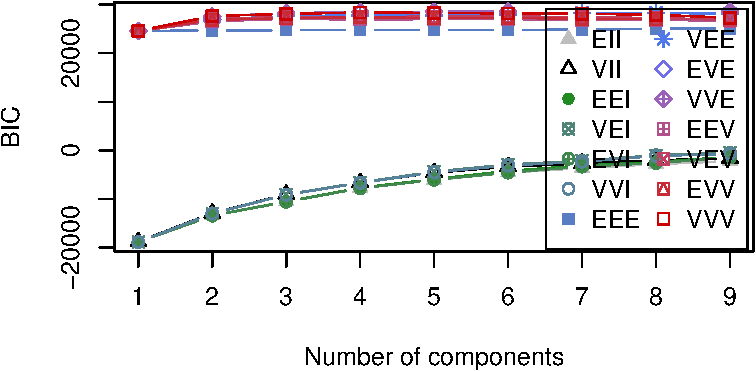
\includegraphics{437_final_project_files/figure-pdf/fig-BIC-1.pdf}

}

\caption{\label{fig-BIC}Visualize the BIC Values For Each K}

\end{figure}

\hypertarget{r-code-used-in-analysis}{%
\subsection{R Code Used in Analysis}\label{r-code-used-in-analysis}}

\begin{verbatim}
\#\# ----load-and-clean-data, message=FALSE, warning=FALSE--------------------------------------------------------
\# Loading Required Packages
library(here)
library(dplyr)
library(mclust)
library(ggplot2)
library(knitr)
library(kableExtra)
library(psych)
library(tidyr)
library(gridExtra)
library(corrplot)

\# Load the RData
load(here("data/CDS_data.RData"))  \# assumes your file is stored in /data

\# Check NAs
\# anyNA(data)

\# Aggregate to 1 row per company
cds_avg <- data %>%
  group_by(Company) %>%
  summarise(across(starts_with("PX"), mean, na.rm = TRUE)) %>%
  ungroup()

\# Log-transform and scale PX1 to PX10
cds_transformed <- cds_avg %>%
  mutate(across(starts_with("PX"), ~ log1p(.))) %>%
  mutate(across(starts_with("PX"), scale))


\#\# ----tbl-data-summary, warning=FALSE, message=FALSE-----------------------------------------------------------
\#| tbl-cap: Summary Statistics of CDS Spread Columns (PX1–PX10)

\# Create summary table
px_summary <- describe(data %>% select(starts_with("PX")))

\# Show as nicely formatted table
kable(px_summary, digits = 2)


\#\# ----fig-box-data---------------------------------------------------------------------------------------------
\#| fig-cap: Distribution of CDS Spreads by Maturity

\# Reshape the data to long formats
data_long <- data %>%
  pivot_longer(cols = starts_with("PX"), names_to = "Tenor", values_to = "Spread")

\# Boxplot of spreads by tenor
ggplot(data_long, aes(x = Tenor, y = Spread)) +
  geom_boxplot(outlier.alpha = 0.2, fill = "lightblue") +
  scale_y_log10() + 
  labs(y = "CDS Spread (log scale)",
       x = "Tenor (PX1–PX10)") +
  theme_minimal()


\#\# ----fig-cor-data, warning=FALSE, message=FALSE---------------------------------------------------------------
\#| fig-cap: Correlation Between CDS Spread Tenors

px_corr <- cor(data %>% select(starts_with("PX")), use = "pairwise.complete.obs")

corrplot(px_corr, method = "color", type = "upper", tl.col = "black", tl.cex = 0.8, mar = c(0, 0, 1, 0))


\#\# ----fit-model, output=FALSE----------------------------------------------------------------------------------
\# Fit Gaussian Mixture Model (GMM)
gmm_model <- Mclust(select(cds_transformed, starts_with("PX")))

\# Add cluster labels to the data
cds_transformed$Cluster <- as.factor(gmm_model$classification)
cds_avg$Cluster <- cds_transformed$Cluster  \# attach to company names


\#\# ----tbl-model-sum--------------------------------------------------------------------------------------------
\#| tbl-cap: GMM Coefficient Summary Table
\# 1. Cluster means (mu_k) — PX1 to PX10 per cluster
cluster_means <- as.data.frame(t(gmm_model$parameters$mean))
cluster_means$Cluster <- rownames(cluster_means)

\# 2. Mixing proportions
cluster_means$Proportion <- round(gmm_model$parameters$pro, 3)

\# 3. Reorder columns
cluster_means <- cluster_means %>%
  relocate(Cluster, Proportion)

\# 4. Format as nice table
kable(cluster_means, caption = "GMM Cluster Means and Mixing Proportions",
      digits = 3, format = "html") %>%
  kable_styling(full_width = FALSE, position = "center")


\#\# ----tbl-cluster-summary--------------------------------------------------------------------------------------
\#| tbl-cap: Number of Companies per GMM Cluster
\# Create a summary table as a data frame
cluster_summary <- as.data.frame(table(cds_avg$Cluster))

\# Rename columns for clarity
colnames(cluster_summary) <- c("Cluster", "Number_of_Companies")

\# Display as kable
kable(cluster_summary, caption = "Number of Companies per Cluster")


\#\# ----fig-cluster----------------------------------------------------------------------------------------------
\#| fig-cap: Clusters of CDS Spread Curves
\#|
\# Visualize PX1 vs PX10 colored by cluster
ggplot(cds_transformed, aes(x = PX1, y = PX10, color = Cluster)) +
  stat_ellipse(geom = "polygon", alpha = 0.1, aes(fill = Cluster), show.legend = FALSE) +
  geom_point(alpha = 0.7) +
  labs(
    x = "Short-Term Spread (PX1)",
    y = "Long-Term Spread (PX10)"
  ) +
  theme_minimal()


\#\# ----fig-trend------------------------------------------------------------------------------------------------
\#| fig-cap: CDS Term Structure by Cluster

\# Reshape data for plotting
library(tidyr)
library(dplyr)
library(ggplot2)

\# Attach cluster labels to original PX values
cds_plot_data <- cds_transformed %>%
  select(starts_with("PX")) %>%
  mutate(Cluster = cds_transformed$Cluster,
         Company = cds_avg$Company) %>%
  pivot_longer(cols = starts_with("PX"), names_to = "Tenor", values_to = "Spread")

\# Plot average PX curve per cluster
cds_plot_data %>%
  group_by(Cluster, Tenor) %>%
  summarise(AvgSpread = mean(Spread), .groups = "drop") %>%
  ggplot(aes(x = Tenor, y = AvgSpread, color = Cluster, group = Cluster)) +
  geom_line(size = 1.2) +
  labs(x = "Tenor (PX1–PX10)",
       y = "Average Transformed Spread") +
  theme_minimal()


\#\# ----fig-boxplot----------------------------------------------------------------------------------------------
\#| fig-cap: Boxplot of Average CDS Spread by Cluster
\# Compute overall average CDS spread per company (across PX1–PX10)
cds_avg$MeanSpread <- cds_avg %>%
  select(starts_with("PX")) %>%
  rowMeans()

\# Boxplot: distribution of risk levels per cluster
ggplot(cds_avg, aes(x = Cluster, y = MeanSpread, fill = Cluster)) +
  geom_boxplot(alpha = 0.7) +
  labs(y = "Average Spread (PX1–PX10)",
       x = "Cluster") +
  theme_minimal()


\#\# ----fig-year-plot,warning=FALSE, message=FALSE---------------------------------------------------------------
\#| fig-cap: Short-Term Risk (PX1) by Cluster Over Time

\# 1. Combine original CDS `data` with cluster labels
data_with_cluster <- data %>%
  group_by(Company) %>%
  mutate(Cluster = cds_transformed$Cluster[match(Company, cds_avg$Company)]) %>%
  ungroup()

\# 2. Convert Date to Date type
data_with_cluster$Date <- as.Date(data_with_cluster$Date)

\# 3. Aggregate: get average PX1 (short-term risk) by Date and Cluster
cds_time_series <- data_with_cluster %>%
  group_by(Date, Cluster) %>%
  summarise(AvgPX1 = mean(PX1, na.rm = TRUE)) %>%
  ungroup()

\# 4. Plot time series
ggplot(cds_time_series, aes(x = Date, y = AvgPX1, color = Cluster)) +
  geom_line(alpha = 0.8, size = 1) +
  labs(title = "Short-Term Risk (PX1) by Cluster Over Time",
       x = "Date",
       y = "Average PX1 (Short-Term CDS Spread)") +
  theme_minimal()


\#\# ----tbl-top-5-companies, warning=FALSE-----------------------------------------------------------------------
\#| tbl-cap: Top 5 Companies from Each Cluster

\# View top 5 companies from each cluster as a kable table
cds_avg %>%
  group_by(Cluster) %>%
  slice_head(n = 5) %>%
  select(Company, Cluster, PX1, PX10) %>%
  kable()


\#\# ----fig-BIC--------------------------------------------------------------------------------------------------
\#| fig-cap: Visualize the BIC Values For Each K

\# Visualize the BIC values for each k
plot(gmm_model, what = "BIC")


\#\# ----appendix-save, message=FALSE, warning=FALSE, echo=FALSE, results='hide'----------------------------------
\# Save the code file silently without showing output
dummy <- knitr::purl("437_final_project.qmd", output = "appendix_code.R")


\#\# ----echo=FALSE, results='asis'-------------------------------------------------------------------------------
knitr::asis_output(
  paste(c("```", gsub("\#", "\\\\\#", readLines("appendix_code.R")), "```"), collapse = "\n")
)
\end{verbatim}

\newpage

\hypertarget{references}{%
\section*{References}\label{references}}
\addcontentsline{toc}{section}{References}

\hypertarget{refs}{}
\begin{CSLReferences}{1}{0}
\leavevmode\vadjust pre{\hypertarget{ref-gridExtra}{}}%
Auguié, Baptiste. 2022. \emph{gridExtra: Functions in Grid Graphics}.
\url{https://CRAN.R-project.org/package=gridExtra}.

\leavevmode\vadjust pre{\hypertarget{ref-here}{}}%
Müller, K. 2023. \emph{Here: A Simpler Way to Find Your Files}.
\url{https://CRAN.R-project.org/package=here}.

\leavevmode\vadjust pre{\hypertarget{ref-citeR}{}}%
R Core Team. 2023. \emph{{R: A Language and Environment for Statistical
Computing}}. Vienna, Austria: R Foundation for Statistical Computing.
\url{https://www.R-project.org/}.

\leavevmode\vadjust pre{\hypertarget{ref-psych}{}}%
Revelle, William. 2024. \emph{Psych: Procedures for Psychological,
Psychometric, and Personality Research}.
\url{https://CRAN.R-project.org/package=psych}.

\leavevmode\vadjust pre{\hypertarget{ref-mclust}{}}%
Scrucca, L., M. Fop, T. B. Murphy, and A. E. Raftery. 2023.
\emph{Mclust: Gaussian Mixture Modelling for Model-Based Clustering,
Classification, and Density Estimation}.
\url{https://CRAN.R-project.org/package=mclust}.

\leavevmode\vadjust pre{\hypertarget{ref-corrplot}{}}%
Wei, Taiyun, and Viliam Simko. 2021. \emph{Corrplot: Visualization of a
Correlation Matrix}. \url{https://CRAN.R-project.org/package=corrplot}.

\leavevmode\vadjust pre{\hypertarget{ref-ggplot2}{}}%
Wickham, Hadley. 2023. \emph{Ggplot2: Elegant Graphics for Data
Analysis}. \url{https://CRAN.R-project.org/package=ggplot2}.

\leavevmode\vadjust pre{\hypertarget{ref-dplyr}{}}%
Wickham, Hadley, Romain François, Lionel Henry, and Kirill Müller. 2023.
\emph{Dplyr: A Grammar of Data Manipulation}.
\url{https://CRAN.R-project.org/package=dplyr}.

\leavevmode\vadjust pre{\hypertarget{ref-tidyr}{}}%
Wickham, Hadley, and Lionel Henry. 2024. \emph{Tidyr: Tidy Messy Data}.
\url{https://CRAN.R-project.org/package=tidyr}.

\leavevmode\vadjust pre{\hypertarget{ref-wikiCDS}{}}%
Wikipedia contributors. 2024. {``Credit Default Swap.''}
\url{https://en.wikipedia.org/wiki/Credit_default_swap}.

\leavevmode\vadjust pre{\hypertarget{ref-knitr}{}}%
Xie, Yihui. 2024. \emph{Knitr: A General-Purpose Package for Dynamic
Report Generation in r}. \url{https://CRAN.R-project.org/package=knitr}.

\leavevmode\vadjust pre{\hypertarget{ref-STA437Notes}{}}%
Zwiernik, Piotr. 2025a. {``Methods for Multivariate Data (STA437).''}
\url{https://pzwiernik.github.io/sta437/}.

\leavevmode\vadjust pre{\hypertarget{ref-STA437}{}}%
---------. 2025b. {``{STA 437/2005: Methods for Multivariate Data}.''}
University of Toronto. \url{https://pzwiernik.github.io/sta437/}.

\end{CSLReferences}



\end{document}
